% ==============================================================================
% Main Manuscript - Nature Publication Standard
% Paper: A Multi-Tissue Transcriptomic Atlas of Porcine Development
% ==============================================================================
\documentclass[11pt,letterpaper]{article}

% ==============================================================================
% PAGE LAYOUT - Nature-compliant margins
% ==============================================================================
\usepackage[
  top=2.5cm,
  bottom=2.5cm,
  left=2.5cm,
  right=2.5cm
]{geometry}

% ==============================================================================
% TYPOGRAPHY - Sans-serif (Helvetica) as required by Nature
% ==============================================================================
\usepackage[T1]{fontenc}
\usepackage{helvet}
\renewcommand{\familydefault}{\sfdefault}
\usepackage{microtype}  % Improved typography

% ==============================================================================
% ESSENTIAL PACKAGES
% ==============================================================================
\usepackage{graphicx}
\usepackage{booktabs}
\usepackage{multirow}
\usepackage{siunitx}
\usepackage{amsmath}
\usepackage{amssymb}
\usepackage[utf8]{inputenc}
\DeclareUnicodeCharacter{03B1}{\ensuremath{\alpha}}
\usepackage{setspace}
\usepackage{caption}
\usepackage{subcaption}
\usepackage{url}
\usepackage{xcolor}
\usepackage{float}
\usepackage{authblk}
\usepackage{enumitem}
\usepackage{lineno}  % Line numbering for peer review

% ==============================================================================
% BIBLIOGRAPHY SETUP - Nature style superscript citations
% ==============================================================================
\usepackage[super,sort&compress,comma]{natbib}
\setlength{\bibsep}{0pt plus 0.3ex}

% ==============================================================================
% COLOR DEFINITIONS
% ==============================================================================
% Removed custom colors to follow standard academic formatting.

% ==============================================================================
% HYPERREF SETUP - Must be loaded late
% ==============================================================================
\usepackage[hidelinks]{hyperref}
\hypersetup{
  colorlinks=true,
  linkcolor=black,
  citecolor=black,
  urlcolor=black,
  pdftitle={A Multi-Tissue Transcriptomic Atlas of Porcine Development},
  pdfauthor={Tianyuan Liu et al.}
}

% ==============================================================================
% AUTHOR FORMATTING - Nature style
% ==============================================================================
\renewcommand\Authfont{\normalsize}
\renewcommand\Affilfont{\small\itshape}
\setlength{\affilsep}{0.5em}
\renewcommand\Authands{, }

% ==============================================================================
% CAPTION FORMATTING - Nature style
% ==============================================================================
\captionsetup{
  font={sf,small},
  labelfont={bf},
  labelsep=colon,
  justification=justified,
  singlelinecheck=false,
  format=plain,
  skip=10pt
}

% ==============================================================================
% LINE SPACING
% ==============================================================================
\onehalfspacing

% ==============================================================================
% FIGURE PLACEMENT
% ==============================================================================
\renewcommand{\floatpagefraction}{0.7}
\renewcommand{\topfraction}{0.9}
\renewcommand{\bottomfraction}{0.9}
\renewcommand{\textfraction}{0.1}

% ==============================================================================
% GRAPHICS PATH
% ==============================================================================
\graphicspath{{figures/output/pdf/}{figures/main/}{figures/supplementary/}}

% ==============================================================================
% CUSTOM COMMANDS
% ==============================================================================
\newcommand{\figref}[1]{Fig.~\ref{#1}}
\newcommand{\tabref}[1]{Table~\ref{#1}}
\newcommand{\secref}[1]{Section~\ref{#1}}
% Note: \eqref is already defined by amsmath

% ==============================================================================
% DOCUMENT METADATA
% ==============================================================================
\title{\textbf{A Multi-Tissue Transcriptomic Atlas of Porcine Development Identifies Conserved Molecular Programs with Humans}}

\author[1,2,3]{Tianyuan Liu}
\author[1]{Rujing Lei}
\author[4]{Ilyas M. Khan}
\author[1,$\ast$]{Peter Theobald}

\affil[1]{Cardiff School of Engineering, Cardiff University, The Parade, Cardiff, CF24 3AA, UK}
\affil[2]{Institute for Integrative Systems Biology (I2SysBio), Spanish National Research Council (CSIC), Paterna 46980, Spain}
\affil[3]{Department of Computer Science, University of Valencia, Spain}
\affil[4]{Faculty of Medicine, Health \& Life Science, Swansea University Medical School, UK}
\affil[$\ast$]{Corresponding author: TheobaldPS@Cardiff.ac.uk}

\date{}

% ==============================================================================
\begin{document}
% ==============================================================================

\linenumbers  % Enable line numbers for peer review

\maketitle

% ==============================================================================
% ABSTRACT
% ==============================================================================
\begin{abstract}
\noindent
Experimental reproducibility and cross-species translation using the domestic pig (\textit{Sus scrofa}) are often limited by the lack of a standardised molecular framework to define biological maturation. The core problem is that while the pig is an excellent preclinical model for human conditions, the molecular tempo of its development is vastly different. Synchronising the maturation rates of \textit{Sus scrofa} and humans is essential to move preclinical research from a descriptive exercise to a predictive science. To address this, we developed a multi-tissue transcriptomic atlas that maps porcine development across five major tissues, providing an objective standard for cross-species synchronization. By applying machine learning to 1,924 RNA-seq profiles, our framework achieves tissue-specific staging (mean balanced accuracy: 0.90 by $K$-fold cross-validation), and identifies highly tissue-specific molecular programs underlying maturation. We provide preliminary cross-species validation through a comparison with human skeletal muscle development ($n = 11$), finding 97\% directional concordance in gene trajectories and a significant correlation ($r = 0.69$, 95\% CI: 0.54--0.80) among 66 conserved developmental genes, including \textit{SORCS2} and \textit{FGFRL1}. These results suggest that porcine molecular maturation shares conserved programs with humans, providing a framework that may enable more accurate cross-species developmental comparisons in nutrition, physiology, and disease modelling.
\end{abstract}

\vspace{1cm}

% ==============================================================================
% INTRODUCTION
% ==============================================================================
\section{Introduction}

The domestic pig (\textit{Sus scrofa}) is central to modern animal science, serving as both a major agricultural species and an increasingly important model organism\cite{swindle_swine_2012,lunney_importance_2021,groenen_analyses_2012}. However, a critical gap undermines reproducibility across pig research: the lack of a standardised, molecular definition of developmental stage. Current staging relies on morphological criteria or chronological age, which are poor proxies for biological maturity\cite{boeyer_evidence_2020}. Littermates frequently develop asynchronously, and distinct organs mature at different rates, effectively decoupling whole-body age from tissue-specific functional competence. This imprecision confounds experimental reproducibility in nutrition, growth physiology, and disease studies, where developmental stage is a critical variable\cite{pluske_gastrointestinal_2018}.

Molecular approaches offer a solution to this challenge. A `universal' epigenetic clock trained on 185 mammalian species\cite{lu_universal_2023}, together with porcine-specific clocks\cite{schachtschneider_epigenetic_2021}, now enables broad translation of biological age between humans and other mammals. Although tissue-specific methylation clocks can be constructed\cite{horvath_dna_2013,duan_epigenetic_2022,teschendorff_epigenetic_2025}, they primarily capture the gradual, cumulative drift of CpG methylation with age rather than the abrupt transcriptional switches that mark developmental phase transitions\cite{hoshino_synchrony_2019}. Epigenetic age can therefore align two species globally while organ-level maturation remains asynchronous---a pig is locomotor-competent at birth, yet its immune and metabolic systems lag behind the corresponding human timeline. Transcriptomic profiling complements methylation-based clocks by providing a direct, functional readout of cellular state, capturing phase-specific gene programs that define tissue maturation\cite{sun_spatial_2025,muralidharan_human_2025}. Yet a comprehensive, tissue-resolved developmental atlas integrating such transcriptomic data has been missing for the pig\cite{bi_ageing_clock_team_multi-tissue_2017,coorens_human_2025}, limiting the standardisation of experimental protocols across research groups.

Here, we present the first multi-tissue transcriptomic atlas of porcine development, integrating data across five major tissues (brain, liver, muscle, lung, and blood) with sufficient sample sizes for machine learning analysis. Unlike previous descriptive studies, we build a quantitative, predictive framework that infers developmental stage with high accuracy directly from gene expression profiles. To assess the biological relevance of our atlas, we performed a preliminary cross-species comparison with human skeletal muscle ($n = 11$), finding a significant positive correlation of developmental trajectories (Pearson $r = 0.69$, 97\% directional concordance) and identifying shared regulatory modules involved in postnatal maturation in both species. We note that cross-species validation is currently limited to muscle tissue due to availability of matched human developmental data. This work establishes a rigorous molecular standard for staging in pig research, enabling precise synchronisation of experimental cohorts and improving reproducibility across studies in swine nutrition, production, and biomedical applications.

% ==============================================================================
% RESULTS
% ==============================================================================
\section{Results}

\subsection{A comprehensive transcriptomic atlas of porcine development}

To define a molecular standard for porcine development, we constructed a large-scale reference atlas using RNA-seq profiles from the PigGTEx resource\cite{teng_compendium_2024,chen_construction_2025,long_comprehensive_2024}, a pig analogue of the human GTEx project\cite{the_gtex_consortium_gtex_2020} (\figref{fig:methodology}a). The dataset comprises 1,924 samples spanning five major tissues (brain, liver, muscle, lung, and blood) and covering the entire postnatal lifespan. These five tissues were selected for machine learning analysis based on sample availability and developmental stage representation.

We addressed the limitations of chronological age by defining five life stages based on physiological milestones: infant (0--20\,d), early childhood (21--59\,d), pre-pubertal (60--149\,d), post-pubertal (150--365\,d), and adult ($>$365\,d) (\figref{fig:methodology}c). These stages correspond to distinct physiological transitions grounded in porcine developmental biology\cite{swindle_swine_2012}: the infant period captures the pre-weaning neonatal phase, during which the gastrointestinal transcriptome undergoes intensive remodelling\cite{inoue_weaning_2015}; early childhood spans the weaning transition (typically 21--28\,d) and its associated gut adaptation\cite{pluske_gastrointestinal_2018}; the pre-pubertal stage encompasses rapid juvenile growth following weaning completion ($\sim$60\,d)\cite{whittemore_whittemores_2006}; the post-pubertal boundary at 150\,d marks the earliest onset of puberty in gilts (reported range: 150--220\,d depending on genetics and management\cite{lents_physiological_2020,swindle_swine_2012}), chosen to capture the molecular preparation for sexual maturation that precedes behavioural oestrus\cite{lents_physiological_2020}; and adulthood ($>$365\,d) represents full reproductive and physiological maturity. This provided a ground truth framework for training, allowing us to decouple ``biological time'' from simple chronological time. The resulting dataset serves as the most comprehensive transcriptomic resource for porcine development to date.

\subsection{Accurate inference of physiological developmental stage}

We implemented a machine learning framework to infer the biological developmental stage directly from tissue-specific transcriptomes (\figref{fig:methodology}b). Models were evaluated using nested cross-validation with automatic hyperparameter tuning to ensure unbiased estimation (see Methods). Pooled held-out performance demonstrated robust generalisation across tissues, with a mean balanced accuracy of 89.5\% across all tissues (\figref{fig:performance}a; see Supplementary Table~S1 for detailed metrics).

Performance varied according to tissue complexity and sample availability. Blood achieved the highest balanced accuracy (95.9\%), followed by liver (92.1\%), muscle (89.4\%), and lung (89.2\%), whereas the brain, with its extreme cellular heterogeneity and limited sample size ($n = 43$), showed lower predictability (81.1\%). Notably, tissues with severe class imbalance required reduced classification schemes (4-class for muscle and liver, 2-class for brain, blood, and lung; \figref{fig:methodology}d) to ensure robust model training (Supplementary Table~S1; Supplementary Fig.~S3a). Consequently, the atlas provides high-resolution multi-stage developmental classification for muscle and liver, but only binary maturity classification (pre-pubertal vs.\ post-pubertal) for brain, blood, and lung; finer staging for these tissues will become feasible as more balanced developmental data accumulates.

Crucially, the system achieved near-perfect ordinal consistency in well-sampled tissues like muscle ($\rho = 0.965$) and liver ($\rho = 0.949$) (\figref{fig:performance}c). The confusion matrices (\figref{fig:performance}b) reveal that ``errors'' largely occurred between adjacent stages (e.g., early vs. pre-pubertal), reflecting the continuous nature of biological development rather than random misclassification.

These tissue-specific performance differences prompted us to ask: what biological programs underlie the model's predictions? To answer this, we examined the functional annotation of the genes that drive accurate stage inference.

\subsection{The functional landscape of development}

Beyond prediction, our model uncovers the biological logic driving maturation. We performed functional enrichment analysis on the top informative genes for each stage, mapping the global landscape of developmental regulation (\figref{fig:biovalidation}).

The resulting functional network reveals that each tissue follows a distinct regulatory framework. In the brain, development is driven by synaptic refinement and metabolic support\cite{kang_spatio-temporal_2011,semple_brain_2013}, highlighted by enrichment of \textit{sarcosine metabolism} (linked to NMDA receptor coagonist availability\cite{zhang_glycine_2009}) and \textit{beta-tubulin binding} (critical for axonal transport). In contrast, the liver prioritises metabolic autonomy and homeostasis, evidenced by the upregulation of \textit{autophagosome-membrane adaptors}. Muscle development centres on contractile machinery assembly and neuromuscular signalling (e.g., \textit{acetylcholinesterase activity}\cite{rotundo_expression_2003}), while the lung focuses on immune system establishment\cite{georgountzou_postnatal_2017} (\textit{IL-6 signalling regulation}) and RNA metabolic remodelling (\textit{m6A reader activity}). This systems-level view moves beyond simple marker genes to capture the coordinated, tissue-specific logic of physiological maturation.

Notably, feature importance rankings showed moderate instability across random seeds (mean Jaccard similarity: 0.08--0.31 across tissues; Supplementary Fig.~S2b), with 6--42\% of top 50 features appearing in $\geq$80\% of runs. This is consistent with the known behaviour of tree-ensemble methods when input features are highly correlated: many distinct feature subsets from co-regulated gene modules can yield equivalent predictions. Importantly, we distinguish between \textit{feature instability} and \textit{model instability}: while the specific genes selected vary across seeds, prediction accuracy is highly stable (e.g., muscle: BA mean = 0.88, std = 0.03 across seeds), confirming that the model captures robust developmental patterns regardless of which specific genes from correlated modules are selected. The selected features showed strong correlations with developmental stage (mean absolute $\rho = 0.2$--$0.6$; Supplementary Fig.~S2c). Critically, cross-tissue feature overlap was extremely low (0.2\% Jaccard similarity). This profound tissue-specificity confirms that each tissue uses unique molecular programs for developmental progression.

\subsection{Evolutionary conservation with human development}

A central question for the pig model is whether its developmental timing biologically mirrors that of humans. We addressed this by performing a direct, quantitative comparison with human skeletal muscle transcriptomes from infant to adult stages\cite{schaiter_molecular_2024,cardoso-moreira_gene_2019} (\figref{fig:crossspecies}). We note that this cross-species validation is limited to muscle tissue due to availability of matched human developmental data.

We found preliminary evidence for conservation of developmental trajectories in muscle tissue. Using pre-specified significance and effect-size criteria (FDR $< 0.10$, Benjamini--Hochberg corrected, and $|\log_2\mathrm{FC}| > 0.5$ in both species; see Methods), we identified 66 genes with significant and biologically meaningful developmental fold-changes in both species. There was a significant positive correlation in fold-changes between species (Pearson $r = 0.69$, $p = 1.09 \times 10^{-10}$, 95\% CI: 0.54--0.80; Supplementary Fig.~S1), with 97.0\% (64/66) of shared developmental markers changing in the same direction (\figref{fig:crossspecies}a). Bootstrap analysis (1,000 iterations) confirmed the robustness of this correlation (95\% CI: 0.50--0.82; Supplementary Fig.~S1b). We note that the correlation magnitude decreases with more permissive FDR thresholds: sensitivity analysis across thresholds from 0.05 to 0.20 showed correlations ranging from $r = 0.61$ to $r = 0.69$ (Supplementary Fig.~S1a), as more permissive thresholds include noisier genes.

We identified three conserved functional modules among the top cross-species markers driving this maturation (\figref{fig:crossspecies}b,c; Supplementary Tables~S3--S4).

\textbf{Module 1: Neuromuscular Maturation and Growth Signalling.} This module comprises genes with high infant expression that decrease during postnatal development, reflecting the transition from active myogenesis to mature muscle homeostasis. \textit{ACHE} (pig FC = $-$3.34, human FC = $-$0.53), essential for neuromuscular junction function\cite{rotundo_expression_2003}, shows elevated expression in the infant stage (0--20\,d; mean TPM = 17.5) that progressively declines to baseline in post-pubertal stages (TPM = 1.3). \textit{SORCS2} (pig FC = $-$4.67, human FC = $-$0.95), a regulator of motor neuron innervation\cite{thomasen_sorcs2_2023}, and \textit{KREMEN1} (pig FC = $-$1.69, human FC = $-$1.43), a Wnt/$\beta$-catenin signalling antagonist\cite{osada_wnt_2006,qin_canonical_2024}, show similar gradual postnatal declines. \textit{NRK} (pig FC = $-$8.56, human FC = $-$2.45), an embryonic Ste20-type kinase expressed predominantly in developing skeletal musculature\cite{kanai-azuma_nrk_1999}, has the second-largest fold change and infant TPM = 128.2 declining to 0.3 in adults. The oncofetal RNA-binding proteins \textit{IGF2BP2} (pig FC = $-$2.19, human FC = $-$2.03) and \textit{IGF2BP3} (pig FC = $-$4.85, human FC = $-$1.23) regulate myoblast proliferation via translational control of growth-related transcripts\cite{li_hmga2-igf2bp2_2012}; their postnatal decline accompanies the transition from proliferative to differentiating myoblasts. \textit{ETV5} (pig FC = $-$2.80, human FC = $-$2.24), a PEA3-subfamily transcription factor implicated in myogenic differentiation and satellite cell activation\cite{taylor_role_1997}. \textit{CCDC8} (pig FC = $-$4.44, human FC = $-$3.14), a core component of the 3M growth-regulatory complex, is implicated in a pathway controlling mammalian growth\cite{hanson_exome_2011}; its downregulation parallels the transition from proliferative to hypertrophic tissue growth.

\textbf{Module 2: Structural Refinement and ECM Remodelling.} This module reflects the transition from rapid tissue growth to structural consolidation, encompassing both cytoskeletal dynamics and extracellular matrix maturation. \textit{FGFRL1} (pig FC = $-$3.03, human FC = $-$2.10) is required for slow muscle fibre development\cite{amann_fgfrl1_2014}; its expression peaks during the infant stage (TPM = 77.4) and drops sharply in early childhood (TPM = 15.6). \textit{DLK1} (pig FC = $-$9.15, human FC = $-$2.88) promotes myogenic differentiation during development\cite{waddell_dlk1_2010,andersen_dual_2013}, with high infant expression (TPM = 338.8) declining sharply as the muscle fiber population matures. \textit{POSTN} (pig FC = $-$7.97, human FC = $-$2.93), a secreted matricellular protein associated with extracellular matrix remodelling during myofibre differentiation and maturation\cite{ozdemir_periostin_2014}, is the most highly expressed ECM gene in this set (infant TPM = 602.4), declining dramatically as tissue architecture stabilises. \textit{ADAMTS2} (pig FC = $-$4.25, human FC = $-$1.83), the principal procollagen N-proteinase\cite{colige_cdna_1997}, and \textit{COL11A2} (pig FC = $-$8.35, human FC = $-$0.70), a collagen component regulating fibril organisation\cite{sun_collagen_2020}, reflect the intensive ECM biosynthesis during rapid postnatal growth. \textit{WDR1} (pig FC = $-$1.69, human FC = $-$0.52), a cofactor of cofilin-mediated actin filament disassembly with critical roles in muscle development\cite{ono_functions_2018}, and \textit{FSCN1} (pig FC = $-$4.28, human FC = $-$1.95), an actin-bundling protein driving cell migration during morphogenesis\cite{adams_roles_2004}, capture the cytoskeletal remodelling required during myofibrillogenesis. \textit{FREM2} (pig FC = $-$4.58, human FC = $-$1.05), a basement membrane protein of the FRAS/FREM complex\cite{kiyozumi_breakdown_2006}, shows postnatal downregulation consistent with the transitional role of the FRAS/FREM complex during embryonic morphogenesis. \textit{TCAF1} (pig FC = $-$4.72, human FC = $-$1.02), which regulates TRPM8 ion channel trafficking and calcium signalling\cite{gkika_trp_2015}, is the highest-importance gene among the cross-species markers (importance = 552.4), with infant TPM = 78.9 declining to 3.0 in adults. \textit{TRIM54}, a muscle-specific E3 ubiquitin ligase that associates with the sarcomeric M-line and Z-line and is required for microtubule stability during myogenesis\cite{gregorio_functional_2005}, shows the opposite pattern---lower infant expression (TPM = 78.3) increasing sharply in early childhood (TPM = 351.1) as the mature contractile apparatus is established.

\textbf{Module 3: Metabolic Transition.} This module captures genes upregulated during metabolic maturation of skeletal muscle. \textit{ME1} (pig FC = 2.59, human FC = 0.64) encodes malic enzyme 1, a key source of NADPH for lipid biosynthesis\cite{simmen_malic_2020}; its expression increases progressively from infant (TPM = 2.8) to adult stages (TPM = 16.9), reflecting the transition from carbohydrate to lipid metabolism. \textit{MAOB} (pig FC = 2.55, human FC = 0.80), a mitochondrial outer membrane enzyme catalysing oxidative deamination of monoamines, shows concordant postnatal upregulation (infant TPM = 5.7 to adult TPM = 33.4), consistent with the general increase in mitochondrial content during postnatal muscle maturation. Notably, \textit{PLA2G4E} (pig FC = 2.32, human FC = $-$1.25), a group~IVE cytosolic phospholipase with calcium-dependent N-acyltransferase activity that generates endocannabinoid precursors, is the only discordant gene among the top 20 markers, showing opposite developmental trajectories in pig and human---potentially reflecting species-specific differences in intramuscular lipid metabolism.

These findings provide preliminary quantitative evidence that pig muscle development shares conserved molecular programs with humans, supporting the use of our transcriptomic atlas as a reference for porcine developmental staging. We note, however, that the current cross-species comparison is limited to infant versus adult expression; a finer-grained alignment across all five porcine stages would require human developmental data with greater age resolution spanning childhood, adolescence, and young adulthood.

% ==============================================================================
% DISCUSSION
% ==============================================================================
\section{Discussion}

We have established the first multi-tissue transcriptomic atlas for porcine development, providing a rigorous molecular alternative to subjective morphological staging\cite{swindle_swine_2012}. By harmonising data across five tissues into a unified predictive framework, we demonstrate that biological maturity can be inferred with high precision solely from gene expression profiles. This shift from qualitative observation to quantitative measurement addresses a long-standing challenge in pig research: the standardisation of developmental staging across experimental cohorts and research groups.

The practical implications for pig research are substantial. Our framework enables researchers to objectively classify animals by biological maturity rather than chronological age, reducing confounding variability in studies of nutrition, growth physiology, and disease susceptibility. For example, when evaluating dietary interventions or growth-promoting treatments, synchronising cohorts by molecular developmental stage rather than age should improve statistical power and reproducibility. The tissue-specific nature of our models also allows researchers to select staging approaches appropriate to their target organ system.

Our staging framework has immediate applications for disease modelling, particularly for age-dependent muscular disorders such as Duchenne Muscular Dystrophy (DMD)\cite{klymiuk_dystrophin-deficient_2013, selsby_porcine_2015}. Since the molecular programs for muscle development appear to be partially conserved between pigs and humans, porcine models may provide superior physiological mirroring compared to rodents. DMD typically manifests in humans between 2--5 years of age\cite{bushby_diagnosis_2010}, with rapid deterioration through the pre-teen years. Using our transcriptomic atlas, this developmental window corresponds approximately to infant stage (0--20\,d) in pigs for early onset, with pathological changes becoming visible by pre-pubertal stage (60\,d) and rapid changes occurring within post-pubertal stage (150\,d). By providing a standardised molecular definition of developmental stages, the atlas enables researchers to identify specific developmentally conserved checkpoints that a successful gene therapy must restore. For example, researchers could track whether a gene therapy successfully stabilises \textit{TRIM54} (microtubule stability) and \textit{FGFRL1} (slow fibre development) expression back to healthy infant or early childhood levels. Critically, by using molecular markers to synchronise experimental cohorts rather than relying on chronological age alone, it may be possible to reduce variability in disease progression and treatment response, improving pre-clinical trial quality.

An important biological finding is the profound tissue-specificity of developmental markers. The extremely low cross-tissue feature overlap (0.2\% Jaccard similarity) reflects genuine biological differences: each tissue uses distinct molecular programs for developmental progression, as evidenced by clear tissue clustering in expression space (Supplementary Fig.~S2a). Within-tissue feature importance rankings showed moderate instability (Jaccard similarity 0.08--0.31; 6--42\% of top 50 features stable across random seeds), which we interpret as biological gene redundancy: developmental genes operate in co-regulated modules, and tree-ensemble methods can select different members of the same functional module across runs while maintaining equivalent predictive performance (BA std $<$ 0.06 across seeds for all tissues). This distinction between feature instability and prediction stability is important: the atlas produces consistent developmental staging regardless of which specific genes from redundant modules are selected.

To assess the biological relevance of our atlas, we performed a preliminary cross-species comparison with human skeletal muscle, identifying three shared regulatory modules---neuromuscular maturation and growth signalling, structural refinement and ECM remodelling, and metabolic transition---comprising 21 genes (including \textit{NRK}, \textit{POSTN}, \textit{IGF2BP2/3}, and \textit{SORCS2}) with conserved developmental trajectories. While the human dataset is small ($n = 11$) and the observed correlation ($r = 0.69$, 95\% CI: 0.54--0.80) is moderate, the 97\% directional concordance and the well-documented biological roles of the identified genes provide supportive evidence that our porcine atlas captures genuine developmental biology rather than species-specific artefacts. Recent work on species-specific developmental tempo provides context for understanding why conserved developmental programs unfold at different rates across species\cite{iwata_metabolic_2024}. However, we emphasise that cross-species validation is currently limited to muscle tissue; extending this analysis to brain, liver, lung, and blood represents a critical future direction.

More broadly, our framework is designed to be species-agnostic: the only required inputs are bulk RNA-seq profiles with age metadata across developmental stages. Epigenetic clocks have demonstrated that biological age prediction can be successfully extended from humans to mice and pigs using DNA methylation\cite{horvath_dna_2013,bi_ageing_clock_team_multi-tissue_2017,schachtschneider_epigenetic_2021}. While those approaches use methylation-based regression, our method applies ordinal machine learning classification to transcriptomic data; nevertheless, the underlying principle---extending biological age frameworks across species---is shared. The growing availability of multi-species developmental transcriptomic resources\cite{cardoso-moreira_gene_2019,coorens_human_2025} provides the data foundation for applying our transcriptomic staging approach to additional livestock and model species, enabling standardised developmental comparisons across agricultural and biomedical research.

We acknowledge the paradox of using chronologically defined bins to train a model intended to capture biological age. In the absence of a ``gold standard'' for physiological maturity, chronological age serves as a noisy proxy. Machine learning theory demonstrates that consistent learning is achievable even with noisy labels, provided appropriate methods are employed\cite{natarajan_learning_2013}; with sufficient data, the resulting model can approximate the true underlying signal---here, the molecular definition of a developmental stage---while being robust to individual labelling noise. Consequently, discrepancies between model prediction and chronological age likely reflect true biological inter-individual variability (developmental acceleration or delay) rather than model error. The fact that the learned molecular signatures (\textit{e.g.}, \textit{SORCS2}, \textit{FGFRL1}) track development in humans, despite vastly different chronological lifespans, strongly supports the conclusion that the model has captured conserved biological programs rather than mere chronological associations.

Several limitations must be acknowledged. First, the PigGTEx dataset aggregates RNA-seq profiles from multiple sequencing platforms and library protocols, which may introduce technical variation. No batch correction was applied prior to modelling because tree-based models are robust to monotonic platform shifts in expression. To directly assess whether cross-project technical variation confounds the developmental signals, we computed gene-level fold-changes within the two largest single-project muscle cohorts (PRJNA488311, $n_{\text{total}} = 81$; PRJNA486202, $n_{\text{total}} = 75$), each spanning four consecutive developmental stages under uniform protocols (see Methods). We repeated this analysis across three developmental contrasts (infant vs.\ early childhood, infant vs.\ pre-pubertal, and infant vs.\ post-pubertal). Within-project fold-changes correlated strongly with full-dataset estimates across all comparisons (pooled Pearson $r = 0.67$--$0.81$; Supplementary Table~S5), and the 66 cross-species validated genes showed high agreement ($r = 0.76$--$0.98$), confirming that the developmental signatures reflect biology rather than batch artifacts even for the earliest and subtlest developmental transitions. Stratified $K$-fold cross-validation ensures all developmental stages are represented in both training and test sets, but does not test cross-project generalisation. Future work should prioritise prospective datasets where individual studies span multiple developmental stages, enabling evaluation of cross-project transferability.

Second, our cross-species validation relies on a small human dataset ($n$ = 11; 4 infants, 7 adults) spanning only two developmental windows---infant and adult---with a substantial age gap that omits critical developmental milestones including adolescence and puberty, preventing a stage-by-stage alignment across all five porcine stages. Third, although the gene selection criteria (FDR $< 0.10$, $|\log_2\mathrm{FC}| > 0.5$) were pre-specified, sensitivity analysis confirms robustness across a range of thresholds. Fourth, class imbalance necessitated reduced classification schemes for some tissues (2-class binary maturity classification for brain, blood, and lung). Fifth, the reliance on bulk RNA-seq averages signals across cell types. Future iterations incorporating single-cell resolution\cite{schaum_single-cell_2018,zheng_measuring_2023} will allow us to dissect precisely which cell populations drive these developmental clocks.

In conclusion, this work provides a transparent, reproducible molecular standard for developmental staging in pig research. The atlas offers an immediately applicable tool for standardising experimental cohorts in swine nutrition, production, and biomedical studies. As the pig continues to serve as a major species for both agricultural and biomedical research, this resource ensures that developmental age is defined with the precision required for rigorous, reproducible science.

% ==============================================================================
% METHODS
% ==============================================================================
\section{Methods}

\subsection{Data acquisition and processing}

Bulk RNA-seq transcript-per-million (TPM) matrices and metadata were obtained from the PigGTEx resource\cite{teng_compendium_2024,chen_construction_2025}. Ages recorded in days were harmonised to developmental stages: infant (0--20\,d), early childhood (21--59\,d), pre-pubertal (60--149\,d), post-pubertal (150--365\,d), and adult ($>$365\,d). Stage boundaries were chosen to align with established physiological milestones in porcine development\cite{swindle_swine_2012}: weaning onset ($\sim$21\,d)\cite{pluske_gastrointestinal_2018}, post-weaning transition completion ($\sim$60\,d)\cite{whittemore_whittemores_2006}, earliest puberty onset ($\sim$150\,d; typical range 150--220\,d)\cite{lents_physiological_2020}, and full maturity ($>$365\,d). Preprocessing consisted of a $\log_2(x+1)$ transformation applied to TPM values. Variance filtering and $z$-score standardisation were omitted because tree-based models are invariant to monotonic transformations and split-based feature selection is unaffected by feature scale.

\subsection{Machine learning framework}

We implemented a reduction-based ordinal classification framework using Light Gradient Boosting Machine (LightGBM)\cite{ke_lightgbm_2017}. Given the ordinal nature of developmental stages ($y \in \{0,\dots,K-1\}$), we decomposed the $K$-class problem into $K-1$ binary classification subtasks (Frank \& Hall method\cite{frank_simple_2001}), where the $k$-th subtask predicts the probability $\Pr(y > k \mid x)$. The final probability for each class $c$ was derived as:
\begin{equation}
\Pr(y = c) = \Pr(y > c-1) - \Pr(y > c)
\label{eq:ordinal_prob}
\end{equation}
where $\Pr(y > -1) = 1$ and $\Pr(y > K-1) = 0$.

Models were trained on all available genes (31,908 per tissue), relying on LightGBM's built-in regularisation for implicit feature selection rather than a separate pre-selection step. Nine hyperparameters were tuned automatically via Optuna\cite{akiba_optuna_2019}: num\_leaves, max\_depth, min\_data\_in\_leaf, learning\_rate, n\_estimators, feature\_fraction, bagging\_fraction, $\lambda_1$ (L1), and $\lambda_2$ (L2). Class weighting was set to \texttt{balanced} and monotone constraints were enforced on the ordinal cumulative models. Each binary sub-model used early stopping (patience = 10) to prevent overfitting.

Models were evaluated using nested cross-validation to ensure unbiased performance estimation. The outer loop employed stratified $K$-fold cross-validation ($K = 5$, automatically reduced for tissues with small class sizes). Within each outer fold, hyperparameters were optimised using an inner 3-fold stratified cross-validation loop with 25 Optuna trials per fold, guided by the Tree-structured Parzen Estimator (TPE) sampler and a median pruner. Held-out predictions from all outer folds were pooled for a single, unbiased estimate of generalisation performance. A final model was then retrained on all available data with hyperparameters tuned via a separate inner cross-validation study. Primary performance metrics included Balanced Accuracy (BA) and Macro-F1 score (Supplementary Fig.~S3; Supplementary Tables~S1 and S2):
\begin{equation}
\mathrm{BA} = \frac{1}{K} \sum_{c=0}^{K-1} \frac{\mathrm{TP}_c}{\mathrm{TP}_c + \mathrm{FN}_c}
\label{eq:ba}
\end{equation}
Confidence intervals (95\%) were calculated using bootstrap resampling (1,000 iterations) on the pooled cross-validated predictions.

\subsection{Cross-species evolutionary analysis}

To quantify developmental conservation, we integrated the pig muscle transcriptomic data with human skeletal muscle developmental RNA-seq profiles from Schaiter \textit{et al.}\cite{schaiter_molecular_2024} (GEO accession GSE257558). Of the larger cohort described in that study, RNA-seq data were available for 11 subjects: 4 infants (ages 7--28 months) and 7 adults (ages 30--56 years), all from quadriceps femoris muscle biopsies. We computed the $\log_2$ fold change of gene expression between infant and adult stages for both species.

Conservation was defined as the Pearson correlation of these developmental fold-change trajectories. We applied pre-specified criteria to select genes: FDR $< 0.10$ (Benjamini--Hochberg corrected) and $|\log_2\mathrm{FC}| > 0.5$ in both species, retaining all genes passing these thresholds (66 genes). No additional selection by feature importance or top-$N$ ranking was applied. We reported the Pearson correlation coefficient with 95\% bootstrap confidence intervals (1,000 iterations). As a robustness check, we performed sensitivity analysis across FDR thresholds from 0.05 to 0.20, confirming consistent positive correlations across the parameter space (Supplementary Fig.~S1a).

\subsection{Within-project batch validation}

To assess whether cross-project technical variation confounds developmental signals, we performed a within-project fold-change validation. We identified the two largest single-project muscle cohorts that each span multiple developmental stages under uniform protocols: PRJNA488311 ($n_{\text{total}} = 81$) and PRJNA486202 ($n_{\text{total}} = 75$), each containing samples from infant through post-pubertal stages. We computed fold-changes across three developmental contrasts, all using infant as the baseline: infant vs.\ early childhood, infant vs.\ pre-pubertal, and infant vs.\ post-pubertal. For each gene and each comparison, we computed $\log_2$ fold change (later stage / infant) and Mann--Whitney $U$ $p$-value, with Benjamini--Hochberg FDR correction, following the same procedure as the cross-species analysis. We then correlated within-project fold-changes with full-dataset fold-changes using Pearson $r$, both genome-wide and for the 66 cross-species validated genes specifically. A pooled within-project estimate was computed by averaging the fold-changes from both projects before correlation. Bootstrap confidence intervals (1,000 iterations) were computed for the pooled correlation at each comparison (Supplementary Table~S5).

\subsection{Functional enrichment}

Gene ontology (GO) enrichment of stage-informative markers was performed using g:Profiler\cite{kolberg_gprofiler-interoperable_2023}, applying a Benjamini--Hochberg FDR correction ($p_{\mathrm{adj}} < 0.05$). We focused on GO Biological Process (BP), KEGG, and Reactome pathway terms to identify physiological functions driving developmental transitions.

% ==============================================================================
% REFERENCES
% ==============================================================================
\bibliographystyle{unsrtnat}
\bibliography{pig-age-human/pig-age-human}

% ==============================================================================
% DATA AVAILABILITY
% ==============================================================================
\section*{Data availability}

The PigGTEx data used in this study is available at \url{https://piggtex.farmgtex.org/}. Raw and processed RNA-seq data are available in the NCBI Gene Expression Omnibus (GEO) under accession number GSE257558.

% ==============================================================================
% CODE AVAILABILITY
% ==============================================================================
\section*{Code availability}

All code required to reproduce the findings is available at \url{https://github.com/TianYuan-Liu/pig-dev-stage}. All analyses were conducted using Python 3.9 and R 4.2.0.

% ==============================================================================
% ACKNOWLEDGEMENTS
% ==============================================================================
\section*{Acknowledgements}

We thank the PigGTEx consortium for providing the transcriptomic data that made this study possible. T.L. was funded by the European Union Marie Sk\l{}odowska-Curie Actions Doctoral Network project LongTREC (HORIZON-MSCA-2021-DN-01 grant agreement project 101072892).

% ==============================================================================
% AUTHOR CONTRIBUTIONS
% ==============================================================================
\section*{Author contributions}

T.L. conceived the study, designed the methodology, performed all computational analyses, interpreted results, and wrote the manuscript. R.L. and I.M.K. contributed to manuscript editing and review. P.T. supervised the study, provided guidance, and edited the manuscript. All authors reviewed and approved the final manuscript.

% ==============================================================================
% COMPETING INTERESTS
% ==============================================================================
\section*{Competing interests}

The authors declare no competing interests.

% ==============================================================================
% ADDITIONAL INFORMATION
% ==============================================================================
\section*{Additional information}

\textbf{Supplementary information} accompanies this paper.

\noindent\textbf{Correspondence} and requests for materials should be addressed to P.T. (TheobaldPS@Cardiff.ac.uk).

\clearpage

% ==============================================================================
% FIGURES
% ==============================================================================
\section*{Figures}
\addcontentsline{toc}{section}{Figures}

% ------------------------------------------------------------------------------
% Figure 1: Study Design
% ------------------------------------------------------------------------------
\begin{figure}[H]
  \centering
  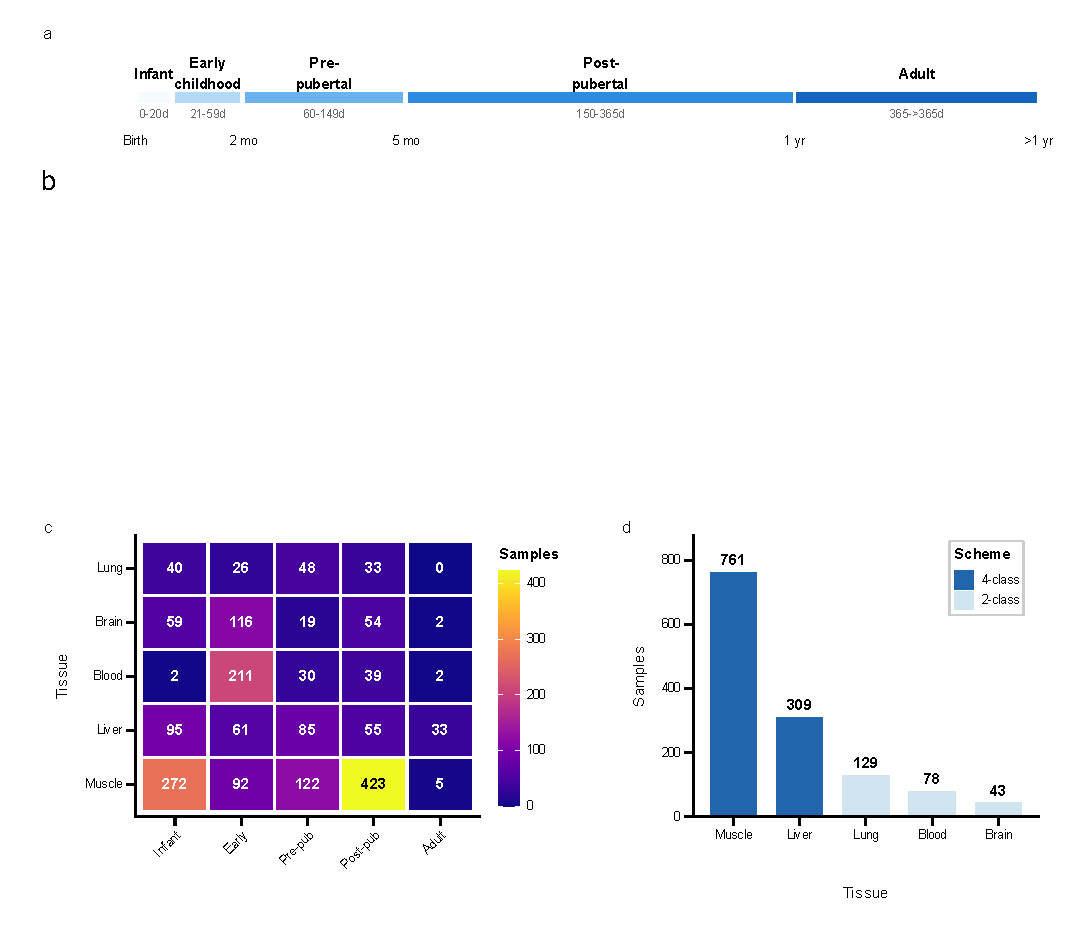
\includegraphics[width=\textwidth]{fig1_study_design.pdf}
  \caption{\textbf{Study design and data landscape.}
  \textbf{a}, Developmental stage definitions mapping chronological porcine age to five ordered stages: infant (0--20\,d), early childhood (21--59\,d), pre-pubertal (60--149\,d), post-pubertal (150--365\,d), and adult ($>$365\,d).
  \textbf{b}, Machine learning workflow diagram illustrating the pipeline from data preprocessing to model calibration and evaluation.
  \textbf{c}, Sample distribution heatmap showing tissue-by-stage availability across 1,924 samples from five tissues.
  \textbf{d}, Classification scheme assignments based on per-class sample availability, with 4-class schemes for muscle and liver, and 2-class schemes for blood, brain, and lung.}
  \label{fig:methodology}
\end{figure}

\clearpage

% ------------------------------------------------------------------------------
% Figure 2: Model Performance
% ------------------------------------------------------------------------------
\begin{figure}[H]
  \centering
  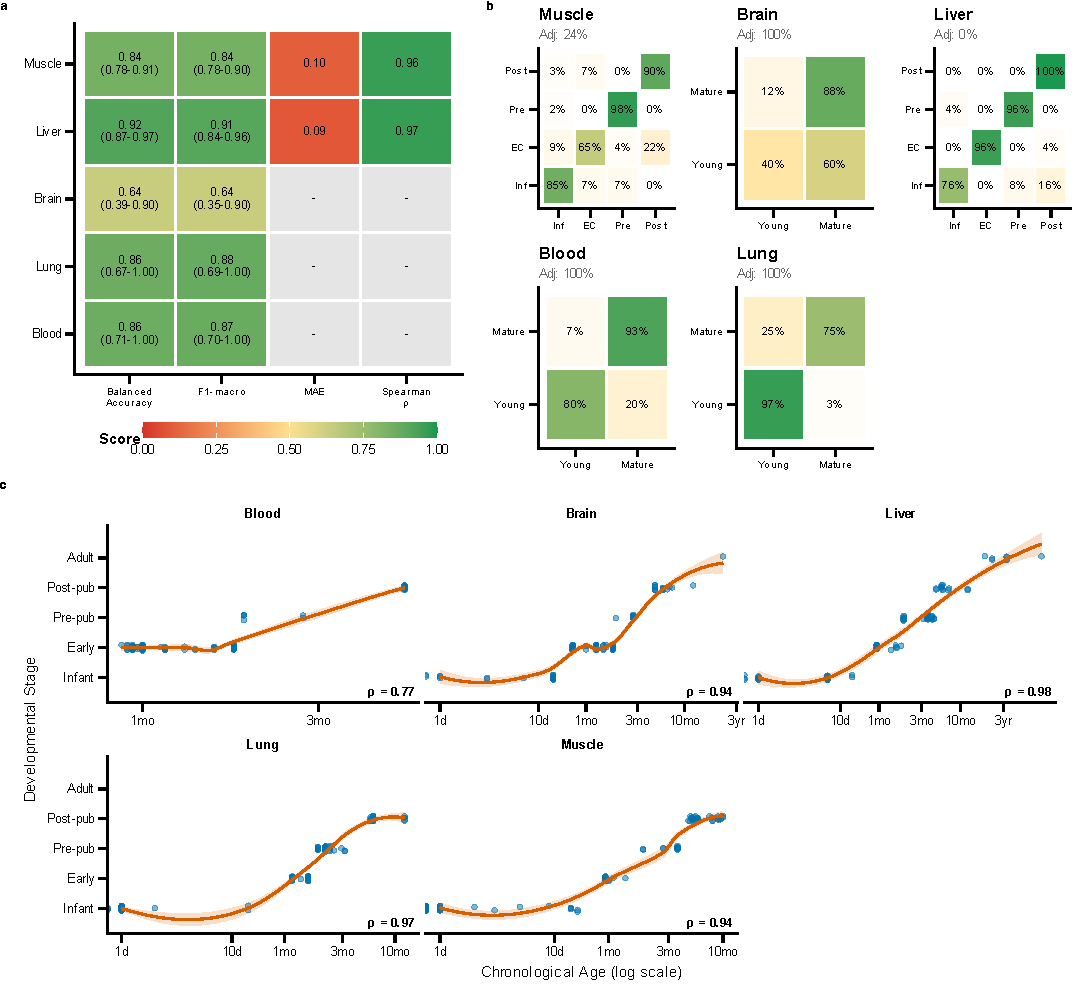
\includegraphics[width=\textwidth]{fig2_model_performance.pdf}
  \caption{\textbf{Classifier performance diagnostics.}
  \textbf{a}, Performance metrics heatmap showing balanced accuracy, macro F1, mean absolute error, and Spearman correlations with 95\% bootstrap confidence intervals across porcine tissues. Mean balanced accuracy across all tissues is 0.895, ranging from 0.811 (brain) to 0.959 (blood).
  \textbf{b}, Confusion matrices for each tissue showing classification accuracy and error patterns.
  \textbf{c}, Scatter plots of predicted developmental stage versus chronological age, demonstrating strong age--stage correlations (muscle $\rho = 0.965$, liver $\rho = 0.949$).}
  \label{fig:performance}
\end{figure}

\clearpage

% ------------------------------------------------------------------------------
% Figure 3: Functional Enrichment
% ------------------------------------------------------------------------------
\begin{figure}[H]
  \centering
  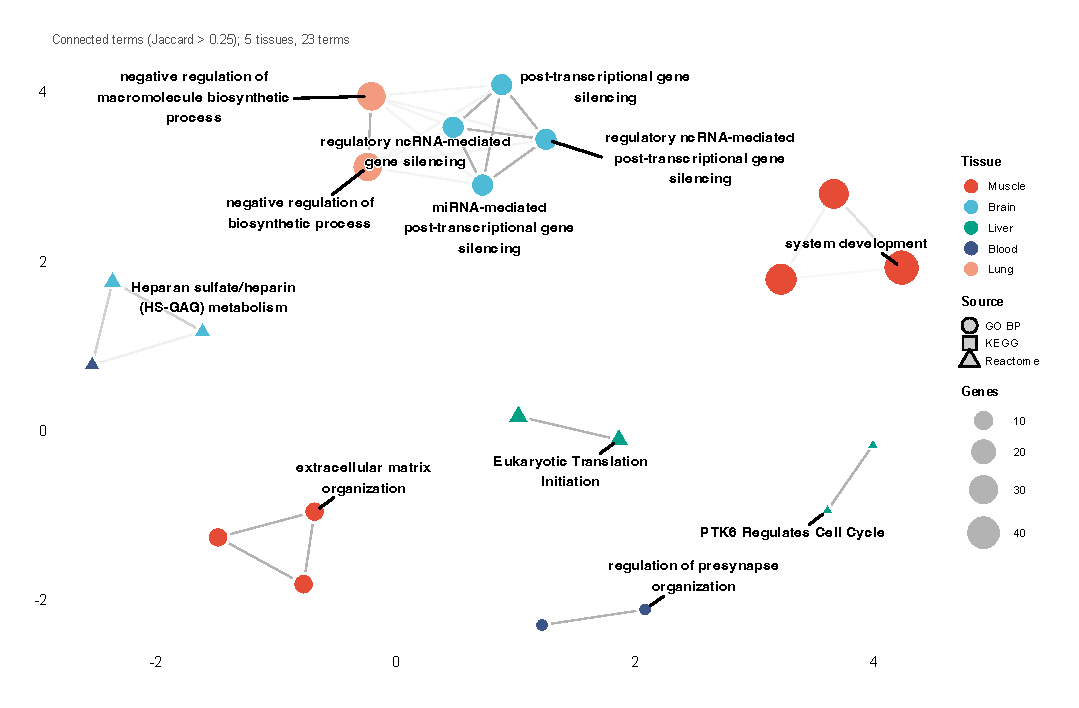
\includegraphics[width=\textwidth]{fig3_functional_enrichment.pdf}
  \caption{\textbf{Functional enrichment analysis of stage-informative porcine genes.}
  Functional network showing interconnected enrichment modules, with nodes representing enriched terms coloured by tissue and edges connecting terms sharing $>$25\% of genes (Jaccard similarity). Hubs and cluster representatives are labelled with biological process or pathway names.}
  \label{fig:biovalidation}
\end{figure}

\clearpage

% ------------------------------------------------------------------------------
% Figure 4: Cross-Species Comparison
% ------------------------------------------------------------------------------
\begin{figure}[H]
  \centering
  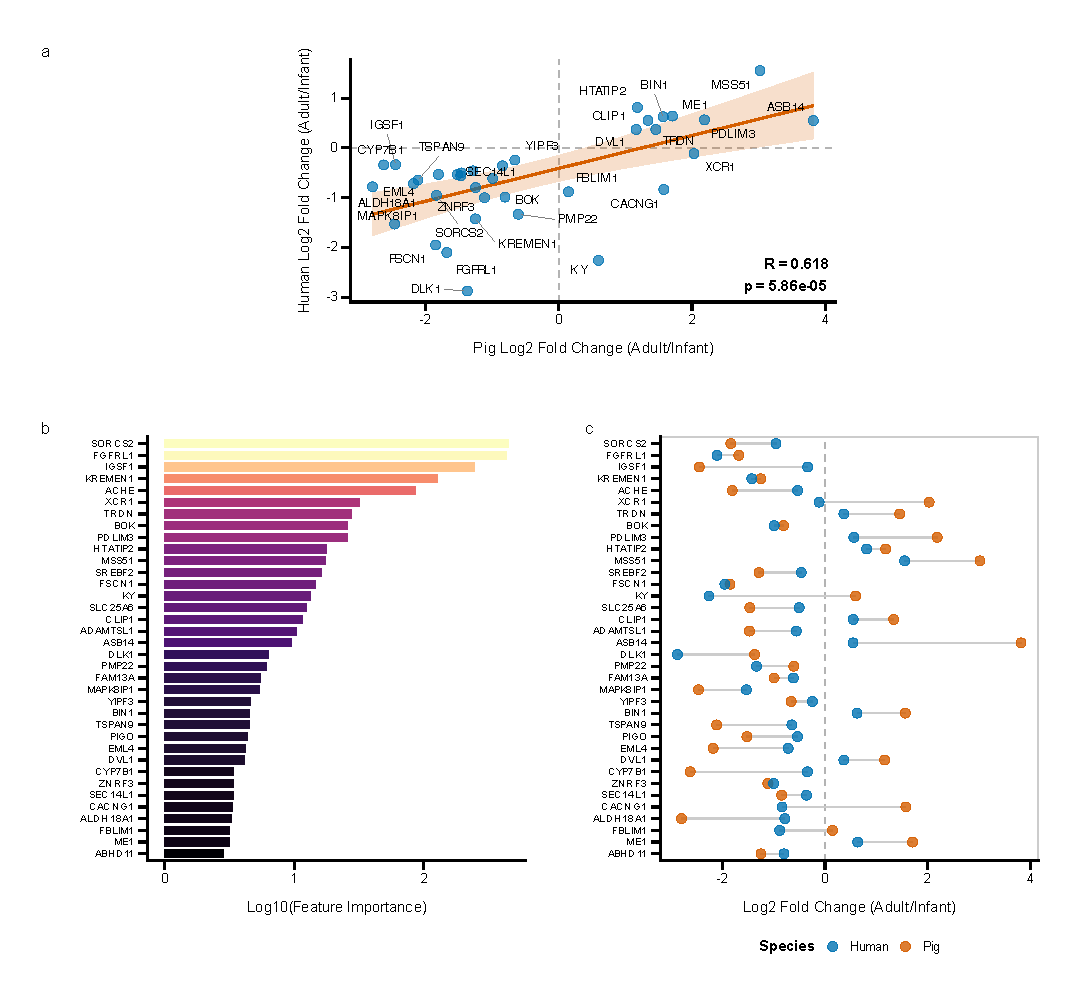
\includegraphics[width=\textwidth,height=0.85\textheight,keepaspectratio]{fig4_cross_species.pdf}
  \caption{\textbf{Cross-species validation of developmental gene expression.}
  Human skeletal muscle transcriptomic data from Schaiter \textit{et al.}\cite{schaiter_molecular_2024} comparing infant (7--28 months) versus adult (30--56 years) samples were used to validate conservation of developmental signatures. For porcine samples, the comparison uses infant stage (0--20\,d) versus post-pubertal/adult stage ($>$150\,d). The five porcine developmental stages are: infant (0--20\,d), early childhood (21--59\,d), pre-pubertal (60--149\,d), post-pubertal (150--365\,d), and adult ($>$365\,d).
  \textbf{a}, Scatter plot of $\log_2$ fold changes between pig and human, showing significant positive correlation (Pearson $r = 0.693$, $p = 1.09 \times 10^{-10}$, 95\% CI: 0.542--0.801). Of 66 genes meeting pre-specified criteria (FDR $< 0.10$, Benjamini--Hochberg corrected, and $|\log_2\mathrm{FC}| > 0.5$) in both species, 64 (97.0\%) showed conserved direction of change.
  \textbf{b}, Feature importance of top conserved markers in the developmental stage classifier.
  \textbf{c}, Paired fold change comparison showing pig and human values for each conserved gene. Top markers include \textit{FGFRL1}, \textit{DLK1}, \textit{KREMEN1}, \textit{ACHE}, and \textit{TCAF1}.}
  \label{fig:crossspecies}
\end{figure}

% ==============================================================================
\end{document}
% ==============================================================================
